\documentclass[a4paper,11.5pt]{article} % тип документа


%%%Библиотеки
	%\usepackage[warn]{mathtext}	
	%\usepackage[T2A]{fontenc} % кодировка
	\usepackage[utf8]{inputenc} % кодировка исходного текста
	\usepackage[english,russian]{babel} % локализация и переносы
	\usepackage{caption}
	\usepackage{listings}
	\usepackage{amsmath,amsfonts,amssymb,amsthm,mathtools}
	\usepackage{wasysym}
	\usepackage{graphicx}%Вставка картинок правильная
	\usepackage{float}%"Плавающие" картинки
	\usepackage{wrapfig}%Обтекание фигур (таблиц, картинок и прочего)
	\usepackage{fancyhdr} %загрузим пакет
	\usepackage{lscape}
	\usepackage{xcolor}
	\usepackage[normalem]{ulem}
	\usepackage{hyperref}

%%%Конец библиотек




%%%Настройка ссылок
	\hypersetup
	{
		colorlinks=true,
		linkcolor=blue,
		filecolor=magenta,
		urlcolor=blue
	}
%%%Конец настройки ссылок


%%%Настройка колонтитулы
	\pagestyle{fancy}
	\fancyhead{}
	\fancyhead[L]{2.4.1}
	\fancyhead[R]{Талашкевич Даниил, группа Б01-009}
	\fancyfoot[C]{\thepage}
%%%конец настройки колонтитулы



							\begin{document}
						%%%%Начало документа%%%%


%%%Начало титульника
\begin{titlepage}

	\newpage
	\begin{center}
		\normalsize Московский физико-технический институт \\(госудраственный 			университет)
	\end{center}

	\vspace{6em}

	\begin{center}
		\Large Лабораторная работа по термодинамике\\
	\end{center}

	\vspace{1em}

	\begin{center}
		\large  \textbf{Определение $\frac{C_p}{C_v}$ методом изобарического расширения газа [2.1.2]}
	\end{center}

	\vspace{2em}

	\begin{center}
		\large Талашкевич Даниил Александрович\\
		Группа Б01-009
	\end{center}

	\vspace{\fill}

	\begin{center}
	Долгопрудный \\12.04.2021
	\end{center}
	
\end{titlepage}
%%%Конец Титульника



%%%Настройка оглавления и нумерации страниц
	\thispagestyle{empty}
	\newpage
	\tableofcontents
	\newpage
	\setcounter{page}{1}
%%%Настройка оглавления и нумерации страниц


					%%%%%%Начало работы с текстом%%%%%%
\section{Аннотация}

\subsection{Цель и оборудование}
\begin{enumerate}
\item \textbf{Цель работь:} определение отношения $C_{p} / C_{v}$ для воздуха или углекислого газа по измерению давления в стеклянном сосуде. Измерения производятся сначала после адиабатического расширения газа, а затем после нагревания сосуда и газа до комнатной темпеpaтypы.

\item \textbf{В работе используются:} стеклянный сосуд; $U$-образный жидкостный манометр; резиновая груша; газгольдер с углекислым газом.
\end{enumerate}

\subsection{Теоретическое введение}

\begin{figure}[h]
	\center{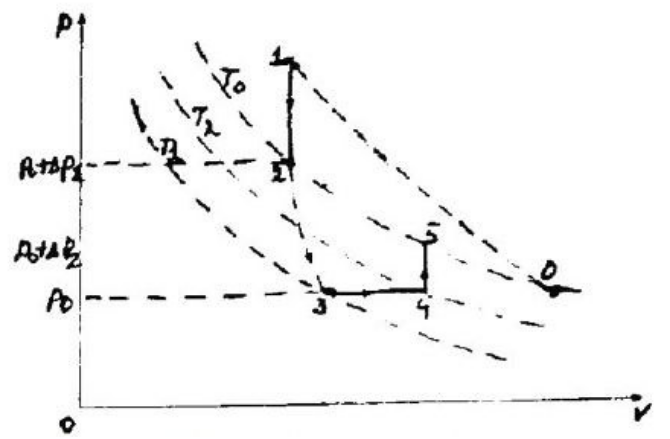
\includegraphics[scale = 0.75]{images/graph_teor.png}}
	\caption{Диаграмма, характеризующая процессы, производимые над воздухом, заключенным в объеме $\Delta V$}
\end{figure}


С помощью резиновой груши, соединённой трубкой с краном $K_1$, в сосуде создаётся заданное избыточное давление $p_1$ воздуха. При этом газ оказывается перегретым, так как совершается работа над газом, соответственно, его внутренняя энергия увеличивается, соответственно, температура тоже увеличивается.

Мысленно выделим в сосуде некоторый объем $\Delta V$ воздуха. Будем следить за изменением его состояния. Вследствие теплообмена со стенками сосуда через некоторое время газ остынет до комнатной температуры $T_0$ (изохорное охлаждение, процесс $1 \longrightarrow 2$ на рис. 2). При этом давление воздуха понизится до $p_0 + \Delta p_1$, где $$\Delta p_1 = \rho g \Delta h_1.~~~~~~~~~~(1)$$
Откроем кран $K$. За время $\Delta t$ порядка 0,5 с произойдёт адиабатическое расширение газа $(2 \longrightarrow 3)$, и его температура окажется ниже комнатной. Далее газ будет изобарически нагреваться (процесс $3 \longrightarrow 4$). Зададим время $\tau$, в течение которого кран $K$ остается открытым, таким чтобы можно было пренебречь временем $\Delta t$ адиабатического расширения воздуха. После закрытия крана газ станет изохорически нагревается до комнатной температуры (процесс $4 \longrightarrow 5$), причём давление внутри возрастет до $p_0 + \Delta p_2$, где $$\Delta p_2 = \rho g \Delta h_2.~~~~~~~~~~(2)$$
Наибольший интерес представляет исследование зависимости отношения перепадов давления $\dfrac{\Delta p_1}{\Delta p_2}$ от времени $\tau$.

С хорошей точностью мы можем считать воздух в идеальным газом. Рассмотрим изобарическое расширение воздуха. Для этого запишем уравнение теплового баланса для изменяющейся со временем массы газа $m = \dfrac{p_0 V_0}{RT} \mu$:
$$c_p m dT = -\alpha (T-T_0)dt,$$
где $c_p$ --- удельная теплоемкость воздуха при постоянном давлении, $\alpha$ --- положительный постоянный коэффициент, характеризующий теплообмен, $V_0$ --- объем сосуда.
$$c_p \dfrac{p_0 V_0}{RT} \mu dT = -\alpha (T-T_0)dt ~~~~~ \text{или} ~~~~~ \dfrac{dT}{T(T - T_0)} = - \dfrac{\alpha dt}{c_p \dfrac{p_0 V_0}{R} \mu}.$$
Заметим, что $\dfrac{1}{T(T - T_0)} = -\dfrac{1}{T_0} \left(\dfrac{1}{T}-\dfrac{1}{T-T_0}\right)$. Тогда $\left(m_0 = \dfrac{p_0 V_0}{RT_0} \mu\right)$:$$\dfrac{1}{T_0} \left(\dfrac{1}{T}-\dfrac{1}{T-T_0}\right) dT = \dfrac{\alpha dt}{c_p m_0 T_0}.$$
После сокращения на $T_0$ выполним интегрирование:
$$\int\limits^{T_2}_{T_1}\left(\dfrac{1}{T}-\dfrac{1}{T-T_0}\right) dT = \dfrac{\alpha}{c_p m_0} \int\limits_0^\tau dt,$$ откуда ($\Delta T_1 = T_1 - T_0,~ \Delta T_2 = T_2 - T_0$): $$\ln \left(\dfrac{T_2}{T_1}\right) - \ln \left(\dfrac{T_2 - T_0}{T_1 - T_0}\right) = \dfrac{\alpha}{c_p m_0} \tau~~~~~\text{или}~~~~~ \ln \left(\dfrac{T_2}{T_1} \dfrac{\Delta T_1}{\Delta T_2}\right) = \dfrac{\alpha}{c_p m_0} \tau.$$
Наконец, $$\dfrac{\Delta T_1}{T_1} = \dfrac{\Delta T_2}{T_2} \exp{\left(\dfrac{\alpha}{c_p m_0} \tau\right)}.~~~~~~~~~~(3)$$
Для адиабатического расширения (процесс $2 \longrightarrow 3$) справедливо данное соотношение: $T^{\gamma} = const \cdot p^{\gamma - 1}$ $\left(\text{здесь}~ \gamma = \dfrac{C_p}{C_v}\right)$. После взятия логарифмических производных получим:
$$\gamma \dfrac{dT}{T} = (\gamma - 1)\dfrac{dp}{p} ~~~~~\text{или}~~~~~\dfrac{dT}{T} = \dfrac{(\gamma - 1)}{\gamma}\dfrac{dp}{p}.$$
Переходя к конечным приращениям найдём:
$$\dfrac{\Delta T_1}{T_1} = \dfrac{(\gamma - 1)}{\gamma}\dfrac{\Delta p_1}{p_0}.~~~~~~~~~~(4)$$
При изохорическом нагреве газа выполняется соотношение: $\dfrac{p}{T} = const$. Возьмём от этого выражения логарифмическую производную: $\dfrac{dp}{p} = \dfrac{dT}{T}$. В конечных приращениях
$$\dfrac{\Delta T_2}{T_2} = \dfrac{\Delta p_2}{p_0}.~~~~~~~~~~(5)$$
После подстановки $(4)$ и $(5)$ в $(3)$ получим:
$$\dfrac{(\gamma - 1)}{\gamma}\dfrac{\Delta p_1}{p_0} = \dfrac{\Delta p_2}{p_0} \exp{\left(\dfrac{\alpha}{c_p m_0} \tau\right)}.$$
Наконец, подставив в это уравнение выражения $(1)$ и $(2)$, получим:
$$\dfrac{(\gamma - 1)}{\gamma} \Delta h_1 = \Delta h_2 \exp{\left(\dfrac{\alpha}{c_p m_0} \tau\right)}~~~~~\text{или}~~~~~\dfrac{\Delta h_1}{\Delta h_2} = \dfrac{\gamma}{\gamma - 1} \exp{\left(\dfrac{\alpha}{c_p m_0} \tau\right)}.$$
Следовательно:
$$\ln \left(\dfrac{\Delta h_1}{\Delta h_2}\right) = \ln \left(\dfrac{\gamma}{\gamma - 1}\right) + \left(\dfrac{\alpha}{c_p m_0} \right) \tau.~~~~~~~~~~(6)$$
Из графика зависимости $\ln \left(\dfrac{\Delta h_1}{\Delta h_2}\right)$ от $\tau$ определим $\gamma$.


\subsection{Эксперементальная установка}

Экспериментальная установка состоит из стеклянного сосуда $A$, снабжённого краном $K_1$, и U-образного жидкостного манометра, измеряющего избыточное давление газа в сосуде. Схема установки показана на рис. 2.

\begin{figure}[!h]
	\center{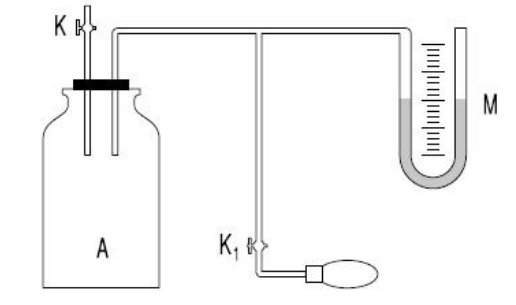
\includegraphics[scale = 0.75]{images/ustan.png}}
	\caption{Установка для определения $\dfrac{C_p}{C_v}$ методом адиабатического расширения газа}
\end{figure}

\newpage

\section{Ход работы}

\subsection{Снятие данных}

На первом этапе будем открывать кран $K_1$ и заполнять сосуд $CO_2$ так, чтобы разность уровней жидкости в манометре составлял $10 \text{см}$, т.~к. для большей разницы мощности газгольдера хватать не будет.

Далее закроем $K_1$, после установления состояния равновесия измерим $\Delta h_1$ и занесем в таблицу.

Потом откроем $K_2$ на время $\tau = 5 \text{с}$. После того, как давление в сосуде перестанет менятся измерим и занесем в таблицу $\Delta h_2$.

Теперь востановим атмосферное давление в сосуде, открыв краны $K_1$ и $K_2$ на $3-4$ минуты.

И повторим так 7 раз, увеличивая время открытия крана $K_2$ до $35 \text{с}$

Теперь построим график $ln\dfrac{\Delta h_1}{\Delta h_2}(\tau)$ и по нему найдем $\gamma$

Полученный график(построенный в MATLAB) приведенен в конце.


\subsection{Аппроксимация полученных данных}

Проведем апроксимирующую прямую ($y = k\cdot x + b$) в программе MATLAB и найдем $b$. Полученное уравнение имеет вид:

\begin{equation}
	y = 0.0529\cdot x + 1.3379
\end{equation}

\begin{equation}
	b = \ln \left(\dfrac{\gamma}{\gamma - 1}\right) \Rightarrow \gamma = \frac{e^b}{e^b - 1} = 1 + \frac{1}{e^b - 1} \Rightarrow \gamma = 1.36
\end{equation}

Рассчитаем погрешности полученной величины в программе MATLAB с помощью формулы:

\begin{equation}
	\sigma_b =\sqrt{\dfrac{1}{n} \cdot \langle\left(\ln \dfrac{\Delta h_1}{\Delta h_2}		\right)^2\rangle - \left(\langle\ln \left(\dfrac{\Delta h_1}{\Delta h_2}\right)\rangle\right)^2 - \ k^2(\langle\tau^2\rangle - \langle\tau\rangle^2)} \Rightarrow \sigma_b = 0.0136
\end{equation} 

Найдем погрешность $b$:

\begin{equation}
	\varepsilon_{b} = \dfrac{\sigma_{b}}{b}\cdot 100 \% = \dfrac{0,0138}{1,3379}\cdot 100 \% =  1,03 \% 
\end{equation} 

Теперь используя погрешность $b$, найдем погрешность требуемой величины:

\begin{equation}
	\sigma_{\gamma} = \gamma \cdot \dfrac{\sigma_{b}}{b}  =  0,02.
\end{equation} 

Найдем относительную погрешность показателя адиабаты для воздуха:

\begin{equation}
	\varepsilon_{\gamma} = \dfrac{\sigma_{\gamma}}{\gamma} = \dfrac{0,02}{1,36}\cdot 100 \% = 1.46\%.
\end{equation} 
 




\subsection{Заключение}

Итогом работы стало получение показателя адиабаты:

\begin{equation}
	\gamma = 1.38 \pm 0.02;   \varepsilon_{\gamma} = 1,46\% 
\end{equation} 

Теперь сравним с табличным значением. Согласно Wikipedia, показатель адиабаты воздуха при $20^{\circ} C$ равен $1.40$, что входит в диапазон погрешности. Это говорит о применимости данного метода для получения показателя адиабаьы воздуха


\section{Графики и таблицы}

\begin{center}
\begin{table}[h]
		\caption{Экспериментальные данные}
\begin{tabular}{|c|c|c|c|c|c|c|c|c|} \hline
$h_{1\text{к}}, \text{мм}$ & $h_{1\text{н}}, \text{мм}$ & $\Delta h_1, \text{мм}$ & $h_{2\text{к}}, \text{мм}$ & $h_{2\text{н}}, \text{мм}$ & $\Delta h_2, \text{мм}$ & $\tau, \text{c}$ & $\dfrac{\Delta h_1}{\Delta h_2}$ & $ln\dfrac{\Delta h_1}{\Delta h_2}$ \\ \hline
22.3 & 14.8 & 7.5 & 18.8 & 17.2 & 1.6 &  5 &  4.69 & 1.54  \\ \hline
22.8 & 13.1 & 9.7 & 18.7 & 17.3 & 1.4 & 10 &  6.93 & 1.94  \\ \hline
22.6 & 13.2 & 9.4 & 18.6 & 17.4 & 1.2 & 15 &  7.83 & 2.06  \\ \hline
22.6 & 13.1 & 9.5 & 18.4 & 17.6 & 0.8 & 20 & 11.88 & 2.47  \\ \hline
22.4 & 13.3 & 9.1 & 18.3 & 17.7 & 0.6 & 25 & 15.17 & 2.72  \\ \hline
22.2 & 13.5 & 8.7 & 18.2 & 17.7 & 0.5 & 30 & 17.40 & 2.86  \\ \hline
22.7 & 13.1 & 9.6 & 18.2 & 17.8 & 0.4 & 35 & 24.00 & 3.18  \\ \hline
\end{tabular}\\\\

\end{table}
\end{center}

\begin{flushleft}

	\begin{figure}[!h]
		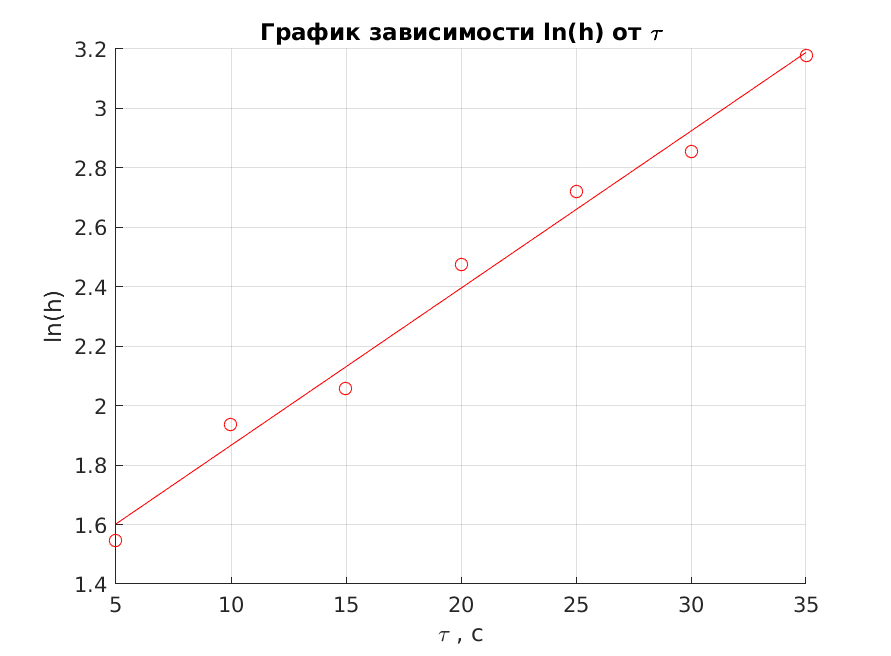
\includegraphics[scale = 0.85]{graph_1.png}
	\end{figure}

\end{flushleft}

\section{Список используемой литературы}

$\bullet$ Гладун А. Д. Лабораторный практикум по общей физике. Термодинамика и молекулярная физика\\

$\bullet$ \href{https://mipt.ru/education/chair/physics/S_II/lab/}{Описание лабораторных работ на кафедре общей физики МФТИ}

\newpage

\end{document}
